\chapter{Pengantar Python}

\section{Serba-serbi python}
\subsection{Apa itu python?}
Python adalah bahasa pemrograman yang multi-paradigma---bisa ditulis dengan konsep prosedural, deklaratif, orientasi obyek, dan fungsional. 

\subsection{Siapa saja pengguna python dan untuk apa?}
Pengguna python sangat banyak, mulai dari \textit{US National Aeronautics and Space Administration} (NASA), Yahoo!, Google, dan banyak lagi. NASA menggunakan python untuk pengembangan dan sebagai bahasa \textit{scripting} dalam berbagai sistemnya, sedangkan Yahoo! dan Google menggunakan python sebagai fondasi dari \textit{search engine} dan bagian dari sistem mereka.

Pertanyaannya seharusnya ``Siapa saja yang tidak menggunakan python?''

\subsection{Kenapa harus menggunakan python?}
``Python Rocks!!''. 

Python memiliki berbagai fitur yang menyebabkan banyak orang memilih python sebagai berikut.
\begin{enumerate}
	\item Cocok untuk pemula
	\\Bandingkan ketiga kode dibawah ini. Manakah yang paling sederhana? 
	\begin{listprog}{Program Hello World dalam C++}
		\label{lst:helloWorldC++}
		\begin{lstlisting}[language=C++]
		#include <iostream>
		using namespace std;
		
		int main{}{
			cout << "Hello World";
			return 0;
		}
		\end{lstlisting}
	\end{listprog}
	\begin{listprog}{Program Hello World dalam Java}
		\label{lst:helloWorldJava}
		\begin{lstlisting}[language=Java]
		public class HelloWorld{
			public static void main(String[] args){
				System.out.println("Hello World");
			}
		}
		\end{lstlisting}
	\end{listprog}
	\begin{listprog}{Program Hello World dalam Python}
		\label{lst:helloWorldPython}
		\begin{lstlisting}[language=Python]
		print "Hello World"
		\end{lstlisting}
	\end{listprog}
	Baik C++ dan Java memerlukan \textit{overhead} dalam listing program mereka seperti misalnya kelas, tipe data, titik koma (;), header, tipe return dan sebagainya. Python sebenarnya juga memiliki semua hal tersebut, tetapi semuanya disembunyikan dalam kesederhanaan bahasa pemrograman. Oleh karena itu, python menjadi pilihan yang tepat bagi mahasiswa ketika mempelajari algoritma tanpa harus terbebani oleh \textit{overhead} listing program yang tidak perlu.
	\item \textit{Python's Integrated Development Environment} (IDLE)
	\\IDLE merupakan lingkungan pemrograman interaktif yang sangat bermanfaat bagi pembelajaran python sendiri. IDLE sudah terinstall secara otomatis ketika menginstall python. Tampilan IDLE bisa dilihat di Gambar \ref{fig:IDLE}. 
	
\begin{figure}[H]
	\centering
		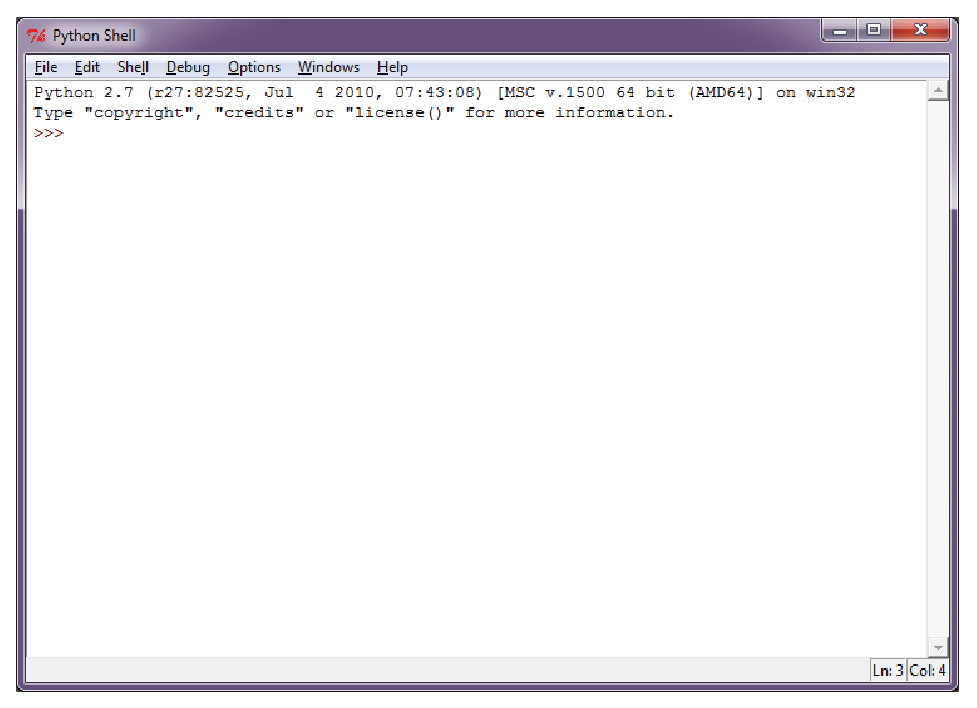
\includegraphics[scale=0.6]{fig/IDLE.eps}
	\caption{Tampilan IDLE}
	\label{fig:IDLE}
\end{figure}

	\item Bilangan bulat besar (\textit{Large Integers})
	\\Python sanggup mengatasi \textit{Large Integers} secara \textit{default} dibandingkan dengan bahasa lain (C++, Java dan lain-lain). 
	Contoh jika diketikkan dalam IDLE:
	\begin{IDLE}
	\\$>>>$ 1987163987163981639186L * 198763981726391826L + 23
	\\\textbf{394976626432005567613000143784791693659L}
	\end{IDLE}
	\item Listing program yang bersih dan indah
	\\Listing program yang dituliskan dengan python lebih gampang dibaca. Python secara \textit{default} memaksa programmer untuk membuat program yang lebih terstruktur (paksaan identasi) dan lebih elegan. Program yang ditulis di python bisa lebih pendek daripada Java ataupun C++. 
	 \begin{listprog}{Menulis teks ke file (Java)}
		\label{lst:tulisTeksJava}
		\begin{lstlisting}[language=Java]
		import java.io.*;
		
		public class IOTest{
			public static void main(String[] args) {
		  	try {
		    	File f = new File("scratch");
		      PrintWriter ps = new PrintWriter(new OutputStreamWriter(new FileOutputStream(f)));
					for (int i = 0; i < 1000000; i++) {
						ps.print(String.valueOf(i));
					}
					ps.close();
				}
				catch(IOException ioe) {
					ioe.printStackTrace();
				}
			}
		}
		\end{lstlisting}
	\end{listprog}
	\begin{listprog}{Menulis teks ke File (Python)}
		\label{lst:tulisTeksPython}
		\begin{lstlisting}[language=Python]
		f=open('scratch','wb')
		for i in xrange(1000000):
			f.write(str(i))
		f.close()
		\end{lstlisting}
	\end{listprog}
	\item Dan masih banyak lagi (dynamically typed, lambda, cocok sebagai tool riset dan lain-lain)
\end{enumerate}

\subsection{Python, versi dan variasi}
Python memiliki banyak variasi dan versi. Python yang digunakan dalam modul ini adalah python yang pertama kali dibuat oleh Guido Von Rossum, yang juga dikenal dengan nama CPython. Adapun implementasi lain dari python adalah sebagai berikut.
\begin{enumerate}
	\item IronPython, implementasi python di .Net Framework.
	\item Jython, implementasi python di Java Virtual Machine
	\item Pypy, python yang lebih cepat dengan JIT compiler.
	\item dan masih banyak lagi.
\end{enumerate}

Kemudian untuk versi python (CPython), tersedia dua versi yang digunakan secara umum yaitu versi 2.x.x (yang terbaru adalah 2.7.x) dan 3.x.x (yang terbaru adalah 3.7.x). Keduanya tidak kompatibel, dan ada perbedaan sintaks yang cukup banyak. 

Python versi 3.x.x (atau python 3) merupakan versi terbaru dari python, akan tetapi masih banyak library yang python versi 2.x.x (atau python 2) yang masih belum di-\textit{porting} ke python 3, maka masih banyak sistem berjalan yang masih menggunakan python 2. 

Untuk informasi lebih lanjut mengenai python 2 vs python 3, bisa dilihat di laman berikut: \url{http://wiki.python.org/moin/Python2orPython3}.

Dalam modul ini masih menggunakan CPython dengan versi 2.7.3. 

\subsection{Installasi python}
Python bisa diunduh di \url{http://python.org/download/}. Di laman tersebut, ada beberapa jenis python yang bisa diunduh. Pilihlah python versi 2.7.x yang sesuai dengan OS yang dipakai (Windows 32-bit---Python 2.7.3 Windows Installer, dan Windows 64-bit---Python 2.7.3 Windows Installer). Untuk Linux, python sudah secara \textit{default} terinstall (versi python tergantung dari distro linux yang digunakan). 

\subsection{IDE python}
Python memiliki banyak IDE yang bisa dipakai. Listing dari IDE yang bisa digunakan untuk CPython bisa dilihat di laman berikut: 
\\\url{http://wiki.python.org/moin/IntegratedDevelopmentEnvironments}. Untuk saat ini, IDE yang paling banyak digunakan adalah pydev (\url{http://pydev.org}). Sebuah IDE lain yang lebih ringan bernama PyScripter \\(\url{http://code.google.com/p/pyscripter}) juga banyak digunakan. 

Untuk menggunakan pydev, lakukan langkah-langkah berikut.
\begin{enumerate}
	\item Unduh Java JDK (jika belum memiliki Java JDK) dari \\\url{http://www.oracle.com/technetwork/java/javase/downloads/index.html}
	\item Install Java JDK  
	\item Unduh eclipse dari \url{http://www.eclipse.org/downloads/}
	\item Installasi pydev di eclipse dengan menggunakan eclipse \textit{update manager}. Cara installasi pydev bisa dilihat di laman \\\url{http://pydev.org/manual_101_install.html}.
\end{enumerate}

Untuk menggunakan PyScripter cukup unduh dari websitenya dan lakukan installasi seperti biasa (harus menginstall python terlebih dahulu). 

\section{Tipe Data Python}

Dalam konteks tipe data python memiliki sifat sebagai beriku.
\begin{enumerate}
	\item \textit{Dynamically Typed}: python akan menentukan secara sendiri tipe data dari setiap variabel yang kita gunakan tanpa harus perlu deklarasi di awal.
	\item \textit{Strongly Typed} yang berarti operasi tertentu hanya bisa dilakukan berdasarkan tipe data yang benar. 
\end{enumerate}

Walaupun python tidak memerlukan secara eksplisit menuliskan tipe data ketika mendeklarasikan variabel, semua variabel yang dideklarasikan tetap termasuk ke dalam tipe data built-in python. Tipe data python bisa dilihat di Table \ref{tbl:tipeDataPython}.

\begin{table}[H]%
\caption{Tipe data built-in}
\centering
\begin{tabular}{|l|l|}
\hline
Tipe Objek & Contoh \\
\hline
Numbers & 111234, 3.1415, 999L, 3+4j, Decimal\\
Strings & 'spam', "guido's"\\
Lists & [1, [2, 'three'], 4]\\
Dictionaries & {'food': 'spam', 'taste': 'yum'}\\
Tuples & (1,'spam', 4, 'U')\\
Files & myfile = open('eggs', 'r')\\
Other types & Sets, types, None, Booleans\\
\hline
\end{tabular}
\label{tbl:tipeDataPython}
\end{table} 

Untuk input dari keyboard, python menggunakan sintaks seperti di Listing \ref{lst:inputPython}
\begin{listprog}{Input di Python (input.py)}
	\label{lst:inputPython}
	\begin{lstlisting}[language=Python]
	umur = input("Berapa umur anda?")
	print "Umur anda adalah: ", umur, "tahun."
	\end{lstlisting}
\end{listprog}

\subsection{String \& Number}

\begin{IDLE}
\begin{tabbing}
$>>>$ a = 4\\
$>>>$ a ~~~~~~~~~~~~~~~~~~~~~~~~~~~~~~~~~~~~ \= \# \textit{Menampilkan hasil dari `a'}\\
\textbf{4}\\
$>>>$ a + 4\\
\textbf{8}\\
$>>>$ a\\
\textbf{4}\\
$>>>$ a = a + 4\\
$>>>$ a\\
\textbf{8}\\
$>>>$ a + 1, a - 1\\ 
\textbf{9,7}\\
$>>>$ a * 3, a / 2 \> \# \textit{Mengalikan dan membagi nilai `a'}\\
\textbf{24,4}\\
$>>>$ a \% 3, a ** 2 \> \# \textit{Modulo dan eksponen nilai `a'}\\
\textbf{2,64}\\
$>>>$ import math \> \# \textit{Import modul math}\\
$>>>$ math.pi \> \# \textit{Menampilkan nilai pi (tidak semuanya)}\\
\textbf{3.1415926535897931}\\
$>>>$ math.sqrt(85) \> \# \textit{Akar dari nilai 85}\\
\textbf{9.2195444572928871} \\
$>>>$ import random \> \# \textit{Import modul random}\\
$>>>$ random.random() \> \# \textit{Menampilkan bilangan acak 0 ~ 1}\\
\textbf{0.3990536432569244}\\
$>>>$ random.choice([23,54,13,44]) \> \# \textit{Memilih salah satu bilangan}\\
\textbf{23}\\
\end{tabbing}
\end{IDLE}

\begin{IDLE}
\begin{tabbing}
$>>>$ S = 'Spam' \\
$>>>$ S ~~~~~~~~~~~~~~~~~~~~~~~~~~~~~~~~~~~~ \= \# \textit{Menampilkan hasil dari `S'}\\
\textbf{'Spam'}\\
$>>>$ len(S) \> \# \textit{Panjang dari `S'}\\
\textbf{4}\\
$>>>$ S[0] \> \# \textit{Karakter pertama dari `S'}\\
\textbf{'S'}\\
$>>>$ S[-1] \> \# \textit{Karakter terakhir dari `S'}\\
\textbf{'m'}\\
$>>>$ S[1:3] \> \# \textit{Irisan S dari karakter 2 sampai 4}\\
\textbf{'pa'}\\
$>>>$ S[1:] \> \# \textit{Irisan S dari karakter 1 sampai habis}\\
\textbf{'pam'}\\
$>>>$ S[:3] \> \# \textit{Irisan S dari awal sampai karakter 3}\\
\textbf{'Spa'}\\
$>>>$ S[:-1] \> \# \textit{Irisan S dari awal sampai karakter 1 dari belakang}\\
\textbf{'Spa'}\\
$>>>$ S[:] \> \# \textit{Semua isi dari S}\\
\textbf{'Spam'}\\
$>>>$ S + 'xyz' \> \# \textit{Penambahan karakter tetapi tidak disimpan ke `S'}\\
\textbf{'Spamxyz}\\
$>>>$ S * 8 \> \# \textit{Repetisi}\\
\textbf{'SpamSpamSpamSpamSpamSpamSpamSpam'}
\end{tabbing}
\end{IDLE}

\subsection{List}

\begin{IDLE}
\begin{tabbing}
$>>>$ L = [123, 'spam', 1.23] ~~~~~~~~~~~~~~~~~~~~~ \= \\
$>>>$ len(L) \> \# \textit{Menampilkan jumlah elemen dari `L'}\\
\textbf{3}\\
$>>>$ L[0]\\
\textbf{123}\\
$>>>$ L[:-1]\\
\textbf{[123, 'spam']}\\
$>>>$ L + [4,5,6]\\
\textbf{[123, 'spam', 1.23, 4, 5, 6]}\\
$>>>$ L.append('NI') \> \# \textit{Menambah elemen 'NI' ke `L'}\\
$>>>$ L \\
\textbf{[123, 'spam', 1.23, 'NI']} \\
$>>>$ L.pop(2) \> \# \textit{Membuang elemen ketiga teratas}\\
\textbf{1.23} \\
$>>>$ L \\ 
\textbf{[123, 'spam', 'NI']} \\
$>>>$ M = [[1,2,3],[4,5,6],[7,8,9]] \> \# \textit{Matriks 3x3}
\end{tabbing}
\end{IDLE}

\subsection{Dictionaries}

\begin{IDLE}
\begin{tabbing}
$>>>$ D = {'food':'Spam', 'quantity':4, 'color':'pink'} \\
$>>>$ D['food'] ~~~~~~~~~~~~~~~~~~~~~~~~~~~~~~~~~~~~~~~~~ \=  \# \textit{Mengambil data}
\textbf{'Spam'} \\
$>>>$ D['quantity'] += 1 \\
$>>>$ D \\ 
\textbf{\{'food': 'Spam', 'color':'pink', 'quantity':5\}} \\
$>>>$ D = \{\} \\
$>>>$ D \\
\textbf{\{\}}\\
$>>>$ D['nama'] = 'Bob' \\
$>>>$ D['pekerjaan'] = 'programmer' \\
$>>>$ D['umur'] = 40 \\
$>>>$ D \\
\textbf{\{'umur': 40, 'pekerjaan':'programmer', 'nama':'Bob'\}}
\end{tabbing}
\end{IDLE}

Kita bisa menggabungkan List, Dictionary dan String dalam salah satu contoh kasus berikut.
\begin{listprog}{Login sederhana(login.py)}
	\label{lst:inputPython}
	\begin{lstlisting}[language=Python]
	Andi = {"username":"andi88","password":"abc"}
	Doni = {"username":"doniyen","password":"123"}
	userdatabase = [Andi,Doni]

	username = input("Masukkan username anda.")
	password = input("Masukkan password anda.")
	login = False
	for user in userdatabase:
	    if (username==user["username"] and password==user["password"]):
	        login = True
	if login: print "Anda berhasil login"
	else: print "Anda gagal login"

	\end{lstlisting}
\end{listprog}

\section{If, Perulangan dan Fungsi}

\subsection{Statement IF}
Format statement IF dalam python bisa ditulis sebagai berikut.

\begin{tabbing}
~~~~~\=if $<$test1$>$:~~~~~~~~~~~~~~~\=\#Pengujian kondisi\\
\>~~~$<$statements1$>$ \> \#Jika True jalankan\\
\>elif $<$test2$>$:\>\#Opsional\\
\>~~~$<$statements2$>$\>\\
\>else:\>\#Opsional\\
\>~~~$<$statements3$>$\>\\
\end{tabbing}

\subsection{Statement FOR}

\begin{tabbing}
~~~~~\=for $<$target$>$ in $<$object$>$:~~~~\=\#Pengujian perulangan\\
\>~~~$<$statements$>$ \> \#Badan perulangan\\
\>~~~if $<$test$>$: break \> \#Keluar dari perulangan\\
\>~~~if $<$test$>$: continue \> \#Kembali ke perulangan\\
\>else:\>\#Opsional\\
\>~~~$<$statements2$>$\> \#Dijalankan jika tidak keluar dari pengulangan dengan BREAK\\
\end{tabbing}

\begin{IDE}
	\begin{listprog}{bubbleSort.py}
		\label{lst:tulisTeksPython}
		\begin{lstlisting}[language=Python]
			A = [4,1,3,5,6,7,2]
			for i in range(1,len(A)):
			    for j in range(i+1):
			        if A[i]<=A[j]:
			            temp = A[i]
			            A[i] = A[j]
			            A[j] = temp
			print A
		\end{lstlisting}
	\end{listprog}		
\end{IDE}

\subsection{Statement WHILE}

\begin{tabbing}
~~~~~\=while $<$test$>$:~~~~~~~~~~~~~~~~~\=\#Pengujian perulangan\\
\>~~~$<$statements1$>$ \> \#Badan perulangan\\
\>~~~if $<$test$>$: break \> \#Keluar dari perulangan\\
\>~~~if $<$test$>$: continue \> \#Kembali ke perulangan\\
\>else:\>\#Opsional\\
\>~~~$<$statements2$>$\> \#Dijalankan jika tidak keluar dari pengulangan dengan BREAK\\
\end{tabbing}

\subsection{Fungsi}

Fungsi pada python menggunakan statement ``def'' dengan format sebagai berikut.
\begin{tabbing}
~~~~~\=def $<$name$>$ (arg1, arg2, \ldots, argN):~~~~\=\#Pengujian perulangan\\
\>~~~\ldots \> \#Badan perulangan\\
\>~~~return $<$value$>$
\end{tabbing}


\begin{IDE}
	\begin{listprog}{fibonacci.py}
		\label{lst:tulisTeksPython}
		\begin{lstlisting}[language=Python]
		def fibonacci(n):
		    if n == 1:
		        return 1
		    elif n == 0:
		        return 0
		    else:
		        return fibonacci(n-1) + fibonacci(n-2)
		
		n = 6
		print "Angka fibonacci ke " + str(n) + " adalah: " + str(fibonacci(n))		
		\end{lstlisting}
	\end{listprog}
\end{IDE}

\begin{IDE}
	\begin{listprog}{FPBEuclid.py}
		\label{lst:tulisTeksPython}
		\begin{lstlisting}[language=Python]
		def euclidFPB(a,b):
	    while b>0:
	        a = a % b 
	        a = a ^ b
	        b = b ^ a 
	        a = a ^ b 
	    return a

		a,b = input("Masukkan angka a dan b:")
		print "Bilangan FPB dari " + str(a) + " dan " + str(b) + " adalah: " + str(euclidFPB(a,b))		
		\end{lstlisting}
	\end{listprog}
\end{IDE}

\subsection{Soal Latihan}

\begin{latihan}
Di bawah ini adalah pseudocode untuk Merge Sort, konversikan ke dalam python dan coba jalankan dengan test case yang anda buat.

\begin{algorithm}[H]
	\caption{MERGE($A,p,q,r$)}
	\label{algo:merge}
	\begin{algorithmic}[1]
		\STATE $n_1 = q - p + 1$
		\STATE $n_2 = r - q$
		\STATE bentuk \textit{array} baru $L[1..n_1+1]$ dan $R[1..n_2+1]$.
		\FOR{$i = 1$ \TO $n_1$}
			\STATE $L[i] = A[p+i-1]$
		\ENDFOR
		\FOR{$j=1$ \TO $n_2$}
			\STATE $R[j] = A[q+j]$
		\ENDFOR
		\STATE $L[n_1+1] = \infty$
		\STATE $R[n_2+1] = \infty$
		\STATE $i=1$
		\STATE $j=1$
		\FOR{$k=p$ \TO $r$}
			\IF{$L[i]\leq{}R[j]$}
				\STATE $A[k] = L[i]$
				\STATE $i = i +1$
			\ELSE
				\STATE $A[k]=R[j]$
				\STATE $j=j+1$
			\ENDIF
		\ENDFOR
	\end{algorithmic}
\end{algorithm}

\begin{algorithm}[H]
	\caption{MERGE-SORT($A,p,r$)}
	\label{algo:mergeSort}
	\begin{algorithmic}[1]
		\IF{$p<r$}
			\STATE $q = \left\lfloor{}(p+r)/2\right\rfloor$
			\STATE MERGE-SORT($A,p,q$)
			\STATE MERGE-SORT($A,q+1,r$)
			\STATE MERGE($A,p,q,r$) 
		\ENDIF
	\end{algorithmic}
\end{algorithm}

\end{latihan}
